\documentclass[dissertation.tex]{subfiles}

\begin{document}

The compiler is comprised of a number of stages and substages, as shown in Figure \ref{fig:compiler-layout}:

\begin{figure}[h]
    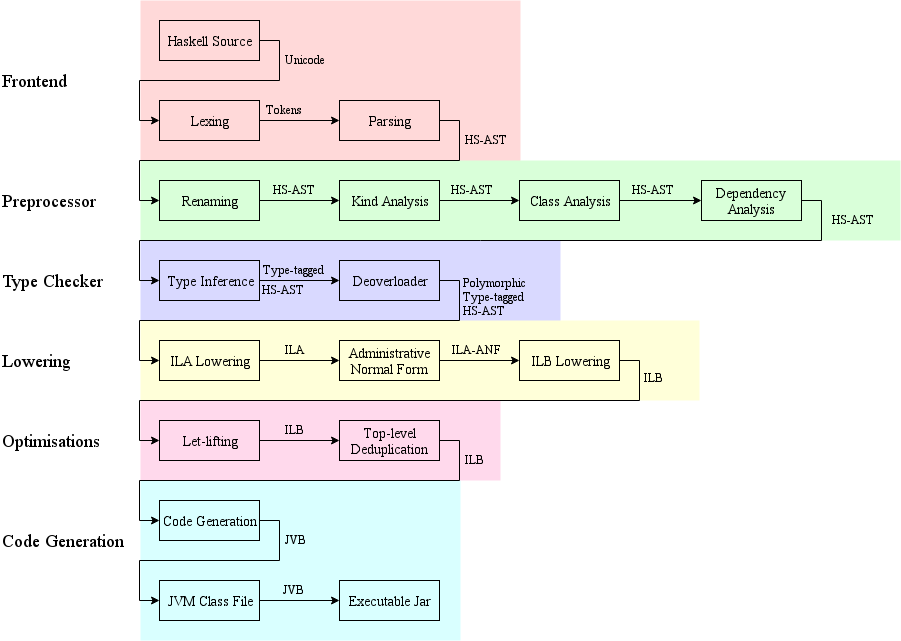
\includegraphics[width=\textwidth]{figures/compiler_layout.png}
    \caption{}
    \label{fig:compiler-layout}
\end{figure}

A brief overview of each stage is given here for a `big picture' view of the compiler, followed by more detailed
descriptions below.

\begin{description}
\item[Frontend]
{
    \hfill

    The frontend consists of standard lexing and parsing from Haskell source code into an Abstract Syntax Tree
    (AST). A modified version of an existing library (haskell-src\footnote{https://github.com/hnefatl/haskell-src})
    is used.

}
\item[Preprocessing]
{
    \hfill
    \begin{itemize}
    \item
    {

        The renamer renames each variable so that later stages can assume each variable name is unique:
        this reduces complexity by removing the possibility of variable shadowing (eg.\ \haskell{let x = 1 in let x
        = 2 in x}).

    }
    \item
    {

        Kind and Class analysis both simply extract useful information about the declarations in the source so that
        stages of the type checker are simpler.

    }
    \item
    {

        Dependency analysis computes a partial order on the source declarations so that the typechecker can process
        them in a valid order.

    }
    \end{itemize}
}
\item[Type Checker]
{
    \hfill
    \begin{itemize}
    \item
    {

        The type inference stage infers polymorphic overloaded types for each symbol, checks them against any
        user-provided type signatures, and alters the AST so that each expression is tagged with its type.

    }
    \item
    {

        Deoverloading converts polymorphic overloaded types to polymorphic types similar to those of System F, and
        alters the AST to implement typeclasses using dictionary-passing.

    }
    \end{itemize}
}
\item[Lowering]
{
    \hfill

    The lowering stage transforms the Haskell source AST into Intermediate Language A (ILA), then rearranges that
    tree into Administrative Normal Form (ILA-ANF), before finally transforming it into Intermediate Language B
    (ILB).

}
\item[Optimisations]
{
    \hfill

    Optimisations transform the intermediate languages while preserving their semantics.

    \todo[inline]{At time of writing these are done on ILB, might change to ILAANF so should update this accordingly.}
    \todo[inline]{If any more optimisations are implemented, update the diagram and here.}

}
\item[Code Generation]
{
    \hfill

    ILB is transformed into Java Bytecode (JVB), and a modified version of an existing library
    (hs-java\footnote{https://github.com/hnefatl/hs-java}) is used to convert a logical representation of the
    bytecode into a set of class files, which are then packaged into an executable Jar file.

}
\end{description}


\section{Implementation Details}
{
    \subsection{Frontend}
    {

        Lexing and parsing of Haskell source is performed using the
        \monospace{haskell-src}\footnote{https://hackage.haskell.org/package/haskell-src} library, which I have modified
        to provide some additional desirable features:

        \begin{itemize}
        \item
        {
            Lexing and parsing declarations for built-in constructors like list and tuple definitions (eg.\
            \haskell{data [] a = [] | a:[a]}).
        }
        \item
        {
            Parsing data declarations without any constructors (eg.\ \haskell{data Int})\footnote{Declarations of this
            form are invalid in the original Haskell 1998 syntax, but valid in Haskell 2010: see
            https://wiki.haskell.org/Empty\_type}. This is a valuable way of introducing built-in types.
        }
        \item
        {
            Adding \haskell{Hashable} and \haskell{Ord} typeclass instances to the syntax AST, so that syntax trees can
            be stored in associative containers.
        }
        \end{itemize}

        The syntax supported is a strict superset of Haskell 1998 and a strict subset of Haskell 2010, but my compiler
        does not have support for all of the features implied by the scope of the syntax. For example, multi-parameter
        typeclasses are parsed correctly as a feature of Haskell 2010 but get rejected by the deoverloading stage.

        \begin{figure}[h]
            \begin{haskellfigure}
            class Convertable a b where
                convert :: a -> b
            instance Convertable Bool Int where
                convert True = 1
                convert False = 0
            \end{haskellfigure}
            \caption{An example of a multi-parameter typeclass}
        \end{figure}

    }
    \subsection{Preprocessor}
    {
        \subsubsection{Renaming}
        {

            Haskell allows for multiple variables to share the same name within different scopes, which can increase the
            complexity of later stages in the pipeline. For example, when typechecking the following code we might
            conflate the two uses of \haskell{x}, and erroneously infer that they have the same type. A similar problem
            arises with variable shadowing, when the scopes overlap. The problem also applies to any type variables
            present in the source -- the type variable \haskell{a} is distinct between the two type signatures:

            \begin{haskellfigure}
            id :: a -> a
            id x = x

            const :: a -> b -> a
            const x _ = x
            \end{haskellfigure}

            Additionally, variables and type variables live in different worlds. The same token can refer to a variable
            and a type variable, even within the same scope -- the following code is perfectly valid (but loops
            forever):

            \begin{haskellfigure}
            x :: x
            x = x
            \end{haskellfigure}

            To eliminate the potential for subtle bugs stemming from this feature, the renamer pass gives each
            semantically distinct variable and type variable in the source a unique name. It traverses the syntax tree
            maintaining a mapping from syntactic variable names to a stack of unique semantic variable names
            (\haskell{Map VariableName [UniqueVariableName]}):

            \begin{itemize}
            \item When a new syntactic variable comes into scope (eg. from a let binding, a lambda argument, a new type signature, a pattern match...), a fresh semantic variable name is generated and pushed onto the stack.
            \item Whenever we leave the scope of a syntactic variable, we pop a semantic name off its corresponding
            stack.
            \item When we see a use of a syntactic variable, we replace it with the current top of the corresponding
            stack.
            \end{itemize}

            A similar mapping is maintained for type variables, with the same rules for maintaining it.

            Type constants such as \haskell{Bool} from \haskell{data Bool = False | True} and typeclass names like
            \haskell{Num} from \haskell{class Num a where ...} are not renamed: these names are already guaranteed to be
            unique by the syntax of Haskell, and renaming them means we need to carry more state through the compiler as
            to what they've been renamed to.

        }
        \subsection{Kind/Class Analysis}
        {

            The typechecker and deoverloader require information about the kinds of any type constructors (the `type of
            the type', eg. \haskell{Int :: *} and \haskell{Maybe :: * -> *}), and the methods provided by different
            classes. This is tricky to compute during typechecking as that pass traverses the AST in dependency order.
            Instead, we just perform a traversal of the AST early in the pipeline to aggregate the required information.

        }
        \subsection{Dependency Analysis}
        {

            When typechecking, the order of processing declarations matters: we can't infer the type of \haskell{foo =
            bar baz} until we've inferred the types of \haskell{bar} and \haskell{baz}. The dependency analysis stage
            determines the order in which the typechecker should process declarations.
            
            We compute the sets of free/bound variables/type variables/type constants for each declaration, then
            construct a dependency graph -- each node is a declaration, and there's an edge from \(A\) to \(B\) if any
            of the bound variables/type variables/type constants at \(A\) are free in \(B\). It is important to
            distinguish between the variables/type variables and type constants, as otherwise name conflicts could occur
            (we don't rename type constants). This separation is upheld in the compiler by using different types for
            each, and is represented in the dependency graph below by colouring symbol names blue or red.
            
            The strongly connected components of the dependency graph correspond to sets of mutually recursive
            declarations, and the partial order between components gives us the order to typecheck each set. For
            example:

            \begin{figure}[H]
                \begin{haskellfigure}
                data Bool = False | True    -- d1
                x = f True                  -- d2
                f y = g y                   -- d3
                g y = h y                   -- d4
                h y = f y                   -- d5
                \end{haskellfigure}
                \caption{}
                \label{code:dependency-graph}
            \end{figure}

            \begin{figure}[H]
                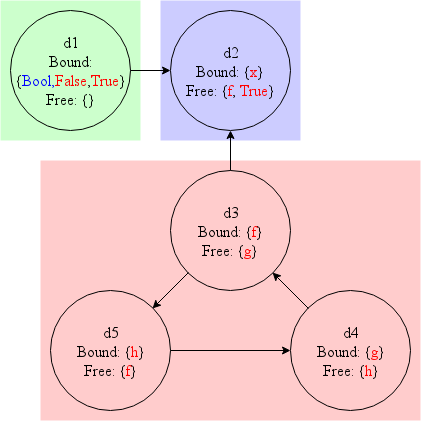
\includegraphics[width=0.5\textwidth]{figures/dependency_graph.png}
                \caption
                {
                    The dependency graph for Figure \ref{code:dependency-graph}. Variables in red, type
                    constants are in blue. Strongly connected components are highlighted.
                }
                \label{fig:dependency-graph}
            \end{figure}

            From the dependency graph, we know we have to typecheck \(d2\) last, after both the trio of functions and
            after the datatype declaration. We also know that we need to typecheck the trio of functions together, as
            they're mutually recursive.

            This process works for languages without ad-hoc overloading, like SML. However, in Haskell there are some
            complications introduced by typeclasses:

            \begin{itemize}
            \item
            {

                Typeclass member variables can be declared multiple times within the same scope. For example:
                
                \begin{haskellfigure}
                class Num a where
                    (+) :: a -> a -> a
                instance Num Int where
                    x + y = ...
                instance Num Float where
                    x + y = ...
                \end{haskellfigure}

                Here the multiple declarations of \haskell{+} don't conflict: this is a valid program. However, the
                following program does have conflicting variables, as \haskell{x} is not a typeclass member and is not
                declared inside an \haskell{instance} declaration:

                \begin{haskellfigure}
                x = True
                x = False
                \end{haskellfigure}

                These declaration conflicts can be expressed in a grid, where:

                \begin{itemize}
                \item
                {
                    
                    \monospace{SymDef |\(x\)|} and \monospace{SymType |\(x\)|} represent top-level declaration and
                    type-signature declarations for a symbol \(x\), like \haskell{|\(x\)| = True} and \haskell{|\(x\)| :: Bool}.

                }
                \item
                {
                    
                    \monospace{ClassSymDef |\(x\)| |\(c\)|} and \monospace{ClassSymType |\(x\)| |\(c\)|} represent
                    \monospace{SymDef |\(x\)|} and \monospace{SymType |\(x\)|} inside the declaration for a class \(c\),
                    like \haskell{class |\(c\)| where { |\(x\)| = True ; |\(x\)| :: Bool }}.

                }
                \item
                {

                    \monospace{InstSymDef |\(x\)| |\(c\)| |\(t\)|} represents a \monospace{SymType |\(x\)|} inside the
                    declaration for a class instance \(c\;t\), like \haskell{instance |\(c\)| |\(t\)| where { |\(x\)| = True }}.

                }
                \end{itemize}

                \begin{figure}[H]
                \small
                \setlength{\tabcolsep}{2pt}
                \begin{tabular}{ l | c c c c c }
                & \texttt{SymDef} \(x_1\) & \texttt{SymType} \(x_1\) & \texttt{ClassSymDef} \(x_1\) \(c_1\) &
                \texttt{ClassTypeDef} \(x_1\) \(c_1\) & \texttt{InstSymDef} \(x_1\) \(c_1\) \(t_1\) \\
                \hline
                \texttt{SymDef} \(x_2\) & \(x_1=x_2\) & \texttt{False} & \(x_1=x_2\) & \(x_1=x_2\) & \(x_1=x_2\) \\
                \texttt{SymType} \(x_2\) & & \(x_1=x_2\) & \(x_1=x_2\) & \(x_1=x_2\) & \(x_1=x_2\) \\
                \texttt{ClassSymDef} \(x_2\) \(c_2\) & & & \(x_1=x_2\) & \(x_1=x_2 \wedge c_1 \neq c_2\) & \(x_1=x_2 \wedge c_1 \neq c_2\) \\
                \texttt{ClassTypeDef} \(x_2\) \(c_2\) & & & & \(x_1=x_2\) & \(x_1=x_2 \wedge c_1 \neq c_2\) \\
                \texttt{InstSymDef} \(x_2\) \(c_2\) \(t_2\) & & & & & \(x_1=x_2 \wedge (c_1 \neq c_2 \vee t_1=t_2)\) \\
                \end{tabular}
                \end{figure}

            }
            \item
            {

                The variables declared within a class declaration are treated as being the binding instance of those
                variables, whereas the declarations of those variables within the instance declarations are treated as
                being free uses of them. This is 

            }
            \item
            {

                Instance usage is actually syntactic not semantic.

            }
            \end{itemize}

        }
    }
}

\end{document}